\documentclass[main]{subfiles}

\begin{document}
    \begin{Reminder}
        \[\text{ряд Лорана } \sum_{n = -\infty}^{+\infty} c_n(z - a)^n  \]
    \end{Reminder}
    \newpage
    \subsection{Изолированные особые точки (однозначного характера). Их классификация. Примеры}
    \begin{Definition}
        \[f \in H(\doted{U}_r(a))\]
        %рисунок1
        \begin{figure}[H]
            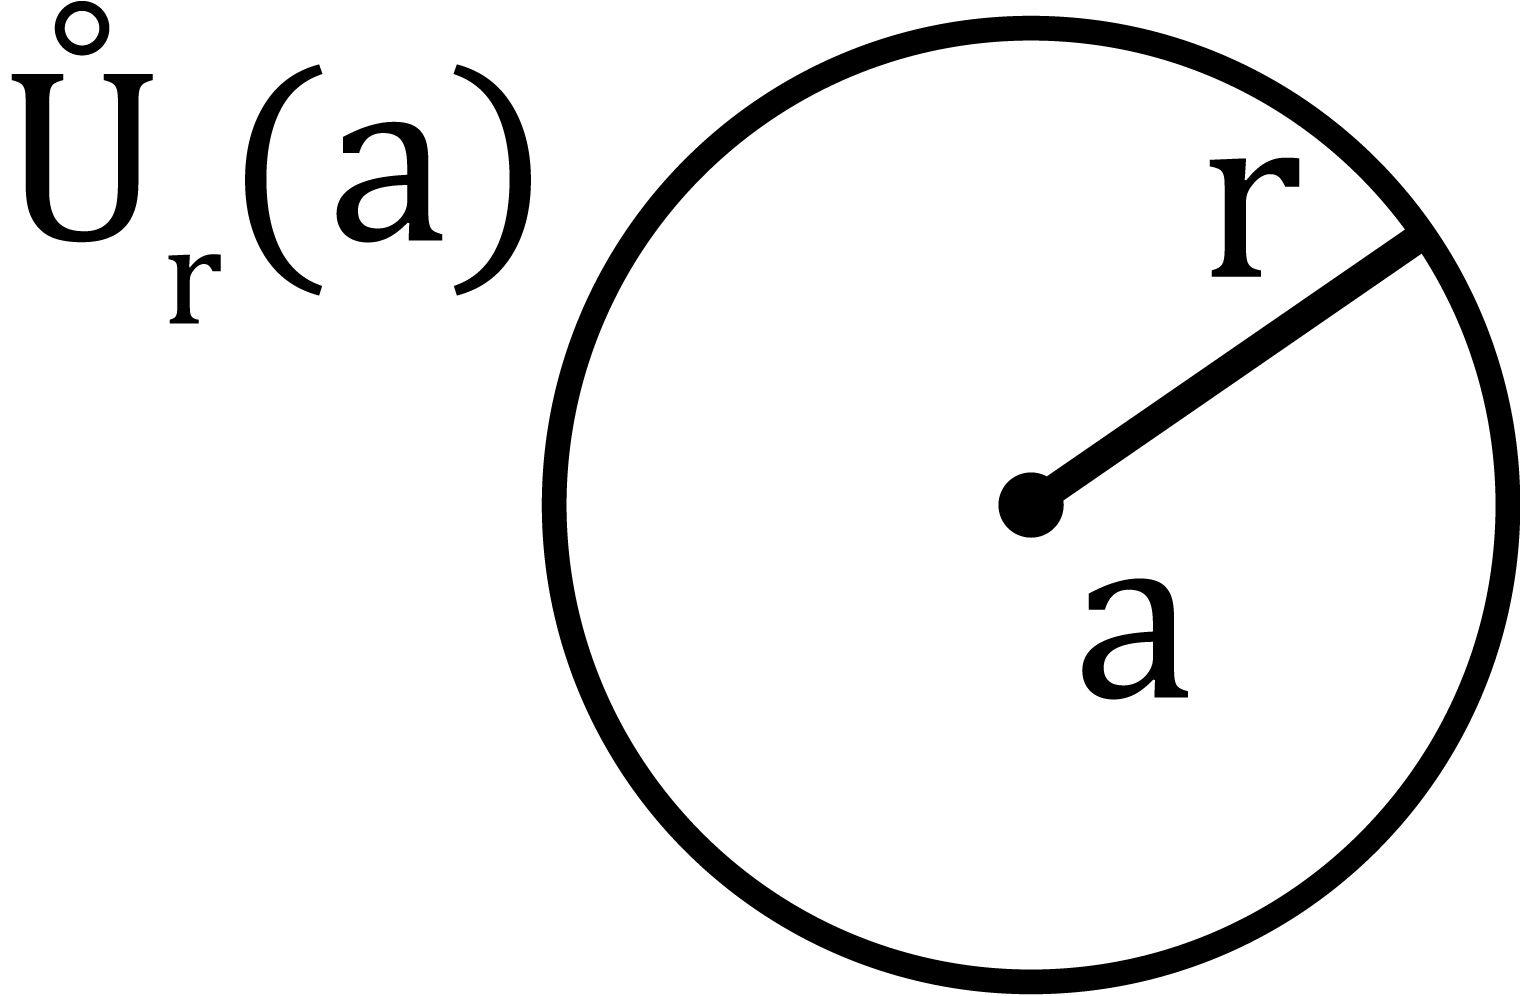
\includegraphics[width=3.5cm]{pics/13_1}
            \centering
        \end{figure}
        \[a \text{ --- устранимая особенность } \rla \text{ р. Л. не содержит слаг. с отр. степ.}\]
        \[\text{т.е } c_{-n} = 0 \q \forall n \in \N \]

        \[a \text{ - уст. ос т.}\]
        \[\Ra  \exists  \lim_{z \to a} f(z) \text{ --- конечный} \]
    \end{Definition}

    \begin{Theorem}[хар-ка устр. ос-сти, Римана]
        \[f \in H(\doted{U}_r(a)) \text{ и огр } \Ra a \text{ --- устр. ос. т}\]
    \end{Theorem}

    \begin{Proof}
        \[\text{Н-ва Коши:} \qq M = \max_{\doted{U}_r(a)} \abs{f(z)} \]
        \[\abs{c_n} \leq M \cdot \rho^{-n} \]
        \[\text{устремим } \rho \to 0\]
        \[\abs{c_{-n} }  \leq M \cdot \rho^n \to 0\]
    \end{Proof}

    \begin{Definition}
        \[a \text{ --- полюс, если } \exists N \in \N: \q \forall n > N \q c_{-n} = 0, \q c_{-N} \neq 0  \]
        \[\frac{c_{-N} }{(z - a)^N} + \frac{c_{-N + 1} }{(z - a)^{N - 1} } + ... + \frac{c_{-1} }
        {z - a} + c_0 + c_1(z - a) + ... + c_k(z - a)^k\]
        конечное число слаг. в гл. части р.Л.
        \[a \text{ - полюс } \rla f(z) \us{z \to a}{\to } \infty\]
        \[f(z) = (z - a)^{-N} (\underbracket{c_{-N} + c_{-N + 1}(z - a) + ... + c_0(z - a)^N + ...  )}_{= h(z)} \]
        \[f(z) = \frac{h(z)}{(z - a)^N}\]
        \[h(a) = c_{-N} \neq 0, \q h \in H(U_r(a)) \]
        \[\frac{1}{f(z)} \to 0 \q \Ra \q f(z) \to \infty\]
    \end{Definition}

    \begin{definition}
        %тут косяк
        Существ. особенность в т.  a $\rla$ гл. часть р. Л. содержит беск ко-во ненул. слаг с отр. степ.
        \[... + \frac{c_{-k} }{(z - a)^k} + ... + \frac{c_{-1} }{(z - a)} + c_0 + c_1(z - a) + ... +
        c_n(z - a)^n + ...\]
        \[\forall N \q \exists n > N: \q c_{-n} \neq 0 \]
    \end{definition}

    \begin{Utv}
        \[\text{a \text{ - существ. особ. т. }} \rla \lim_{z \to a} f(z) \ \cancel{\exists } \]
    \end{Utv}

    \begin{Example}[1]
        \[\text{Устр. особ. т. } f(z) = \frac{\sin z}{z} \qq a = 0 \]
        \[\frac{\sin z}{z} = \frac{z - \frac{z^3}{3!} + ... + (-1)^n \frac{z^{2n + 1} }{(2n + 1)!} + ... }{z} =
        1 - \frac{z^2}{3!} + \frac{z^4}{5!} + ... + \frac{(-1)^n z^{2n} }{(2n + 1)!} + ...\]
        Нет слаг. с отр. степ. \q $c_{-n} = 0, \q n \in \N$ \\
        С другой стороны
        \[\exists \lim_{z \to 0} \frac{\sin z}{z} = 1 \]
    \end{Example}

    \begin{Example}[2.а полюс]
        \[f(z) = \frac{1}{(z - 1)^2} + \frac{1}{(z - 1)} - 8 + (z - 1)^5\]
        Полюс пор. 2 в т $a = 1$
        \[\lim_{z \to 1} f(z) = \infty \]
    \end{Example}

    \begin{Example}[2.б полюс]
        \[f(z) = \frac{1}{\sin z}, \q a = 0 \text{ --- полюс}\]
        \[\text{т.к. } \lim_{z \to 0} \frac{1}{\sin z} = \infty \]
        Какого порядка полюс?\\
        Если $a$ --- пол. порядка $n \q f(z)$, то $a - $ ноль кр. $n \q \frac{1}{f(z)}$
        \[f(z) = \frac{h(z)}{(z - a)^n}, \q h(a) \neq 0 \q \rla \q \frac{1}{f(z)} = \frac{(z - a)^n}{h(z)}\]
        \[a \text{ - ноль кр. } n \q \frac{1}{f(z)}, \text{ т.к. }
        \left(\frac{1}{f(z)}\right)^{(k)} = 0 \qq \forall k \leq n - 1 \]
        \[\left(\frac{1}{f(z)}\right)^{(n)} \neq 0 \]
        \[\frac{1}{f(z)} = \sin z\]
        \[\left(\frac{1}{f(z)}\right)'\bigg|_{a = 0} = \cos z\bigg|_{a = 0} = 1 \neq 0  \]
        \[\text{т.о. } a = 0 \text{ - пол. порядка } 1\]
        УПР $f(z) = \frac{1}{\cos z - 1} \qq a = 0 ?$
    \end{Example}

    \begin{Example}[3 сущ. ос-ть]\
        %рисунок2
        \begin{figure}[H]
            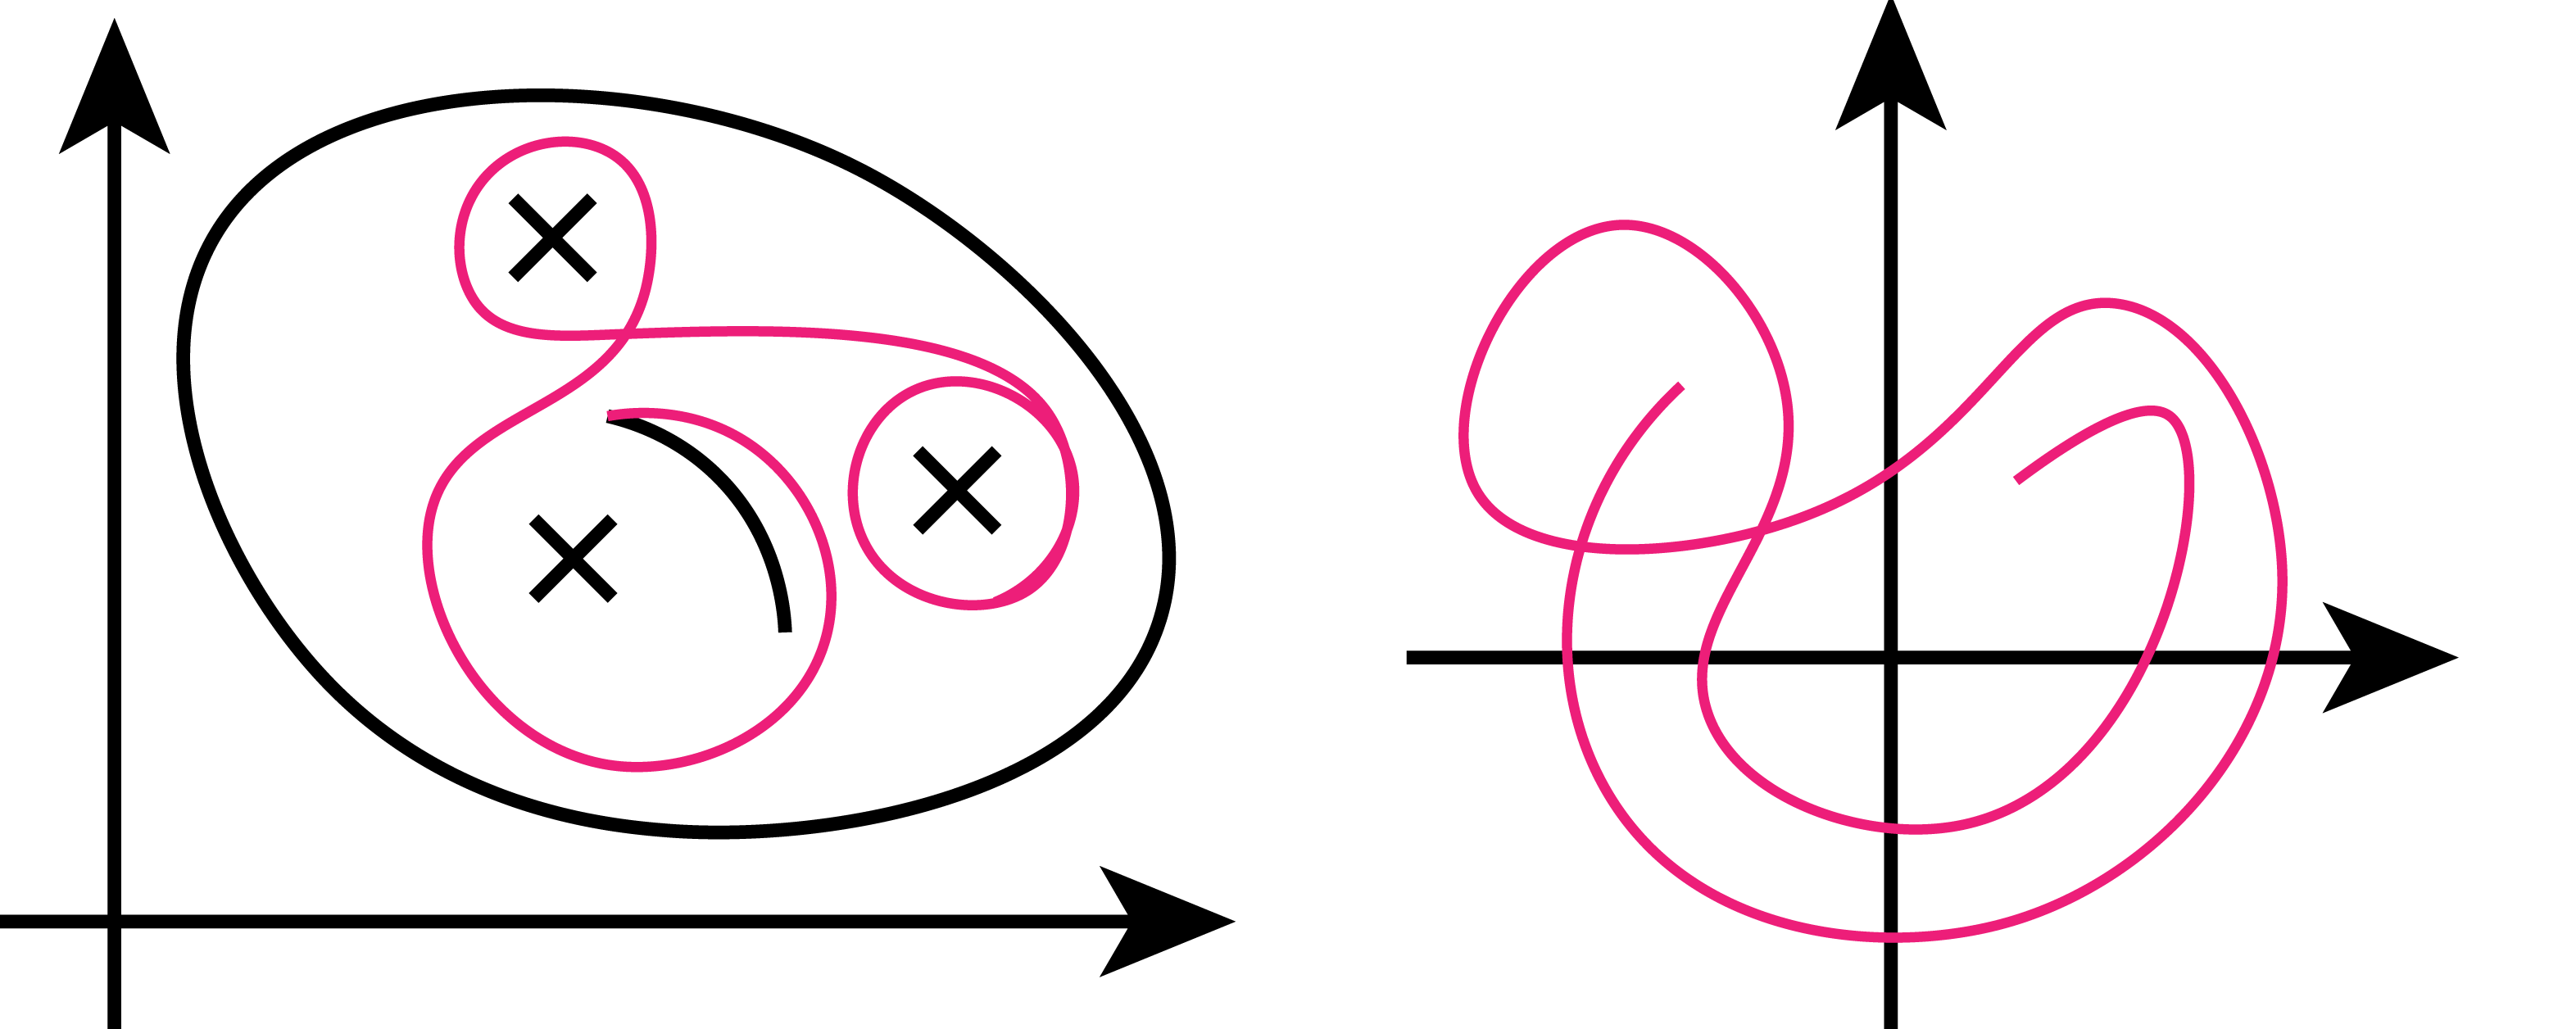
\includegraphics[width=3cm]{pics/13_2}
            \centering
        \end{figure}
        \[f(z) = \cos \frac{1}{z} \qq a = 0\]
        \[\cos \frac{1}{z} = 1 - \frac{1}{z^2 \cdot 2!} + \frac{1}{z^4 \cdot 4!} - ... +
        (-1)^n \frac{1}{z^{2n}(2n)! } + ...\]
        гл. часть содержит бесконечное число слаг.\\
        \[z_k = \frac{1}{2\pi k} \us{k \to \infty}{\to } 0 \qq f(z_k) = 1 \us{k \to \infty}{\to } 1\]
        с др. стороны
        \[\widetilde{z}_k = \frac{1}{2\pi k + \frac{\pi}{2}} \us{k \to \infty}{\to } 0\qq
        f(\widetilde{z}_k) = 0 \us{k \to \infty}{\to } 0\]
        Из определения по Гейне и т. о ед пред. $\Ra $ предела $\cancel{\exists }$\\
        УПР: $z^*_k : \ z_k^* \to  0, \q f(z_k^*) \to 3?$
    \end{Example}

    \newpage
    \subsection{Вычет. Вычисление вычета в различных случаях}

    \begin{Definition}
        \[f \in H(\doted{U}_r(a))\]
        \[res_a f = \frac{1}{2\pi i}\int_{\abs{z - a} = \delta} f(\xi)d\xi , \q 0 < \delta < r \]
        %рисунок3
        \begin{figure}[H]
            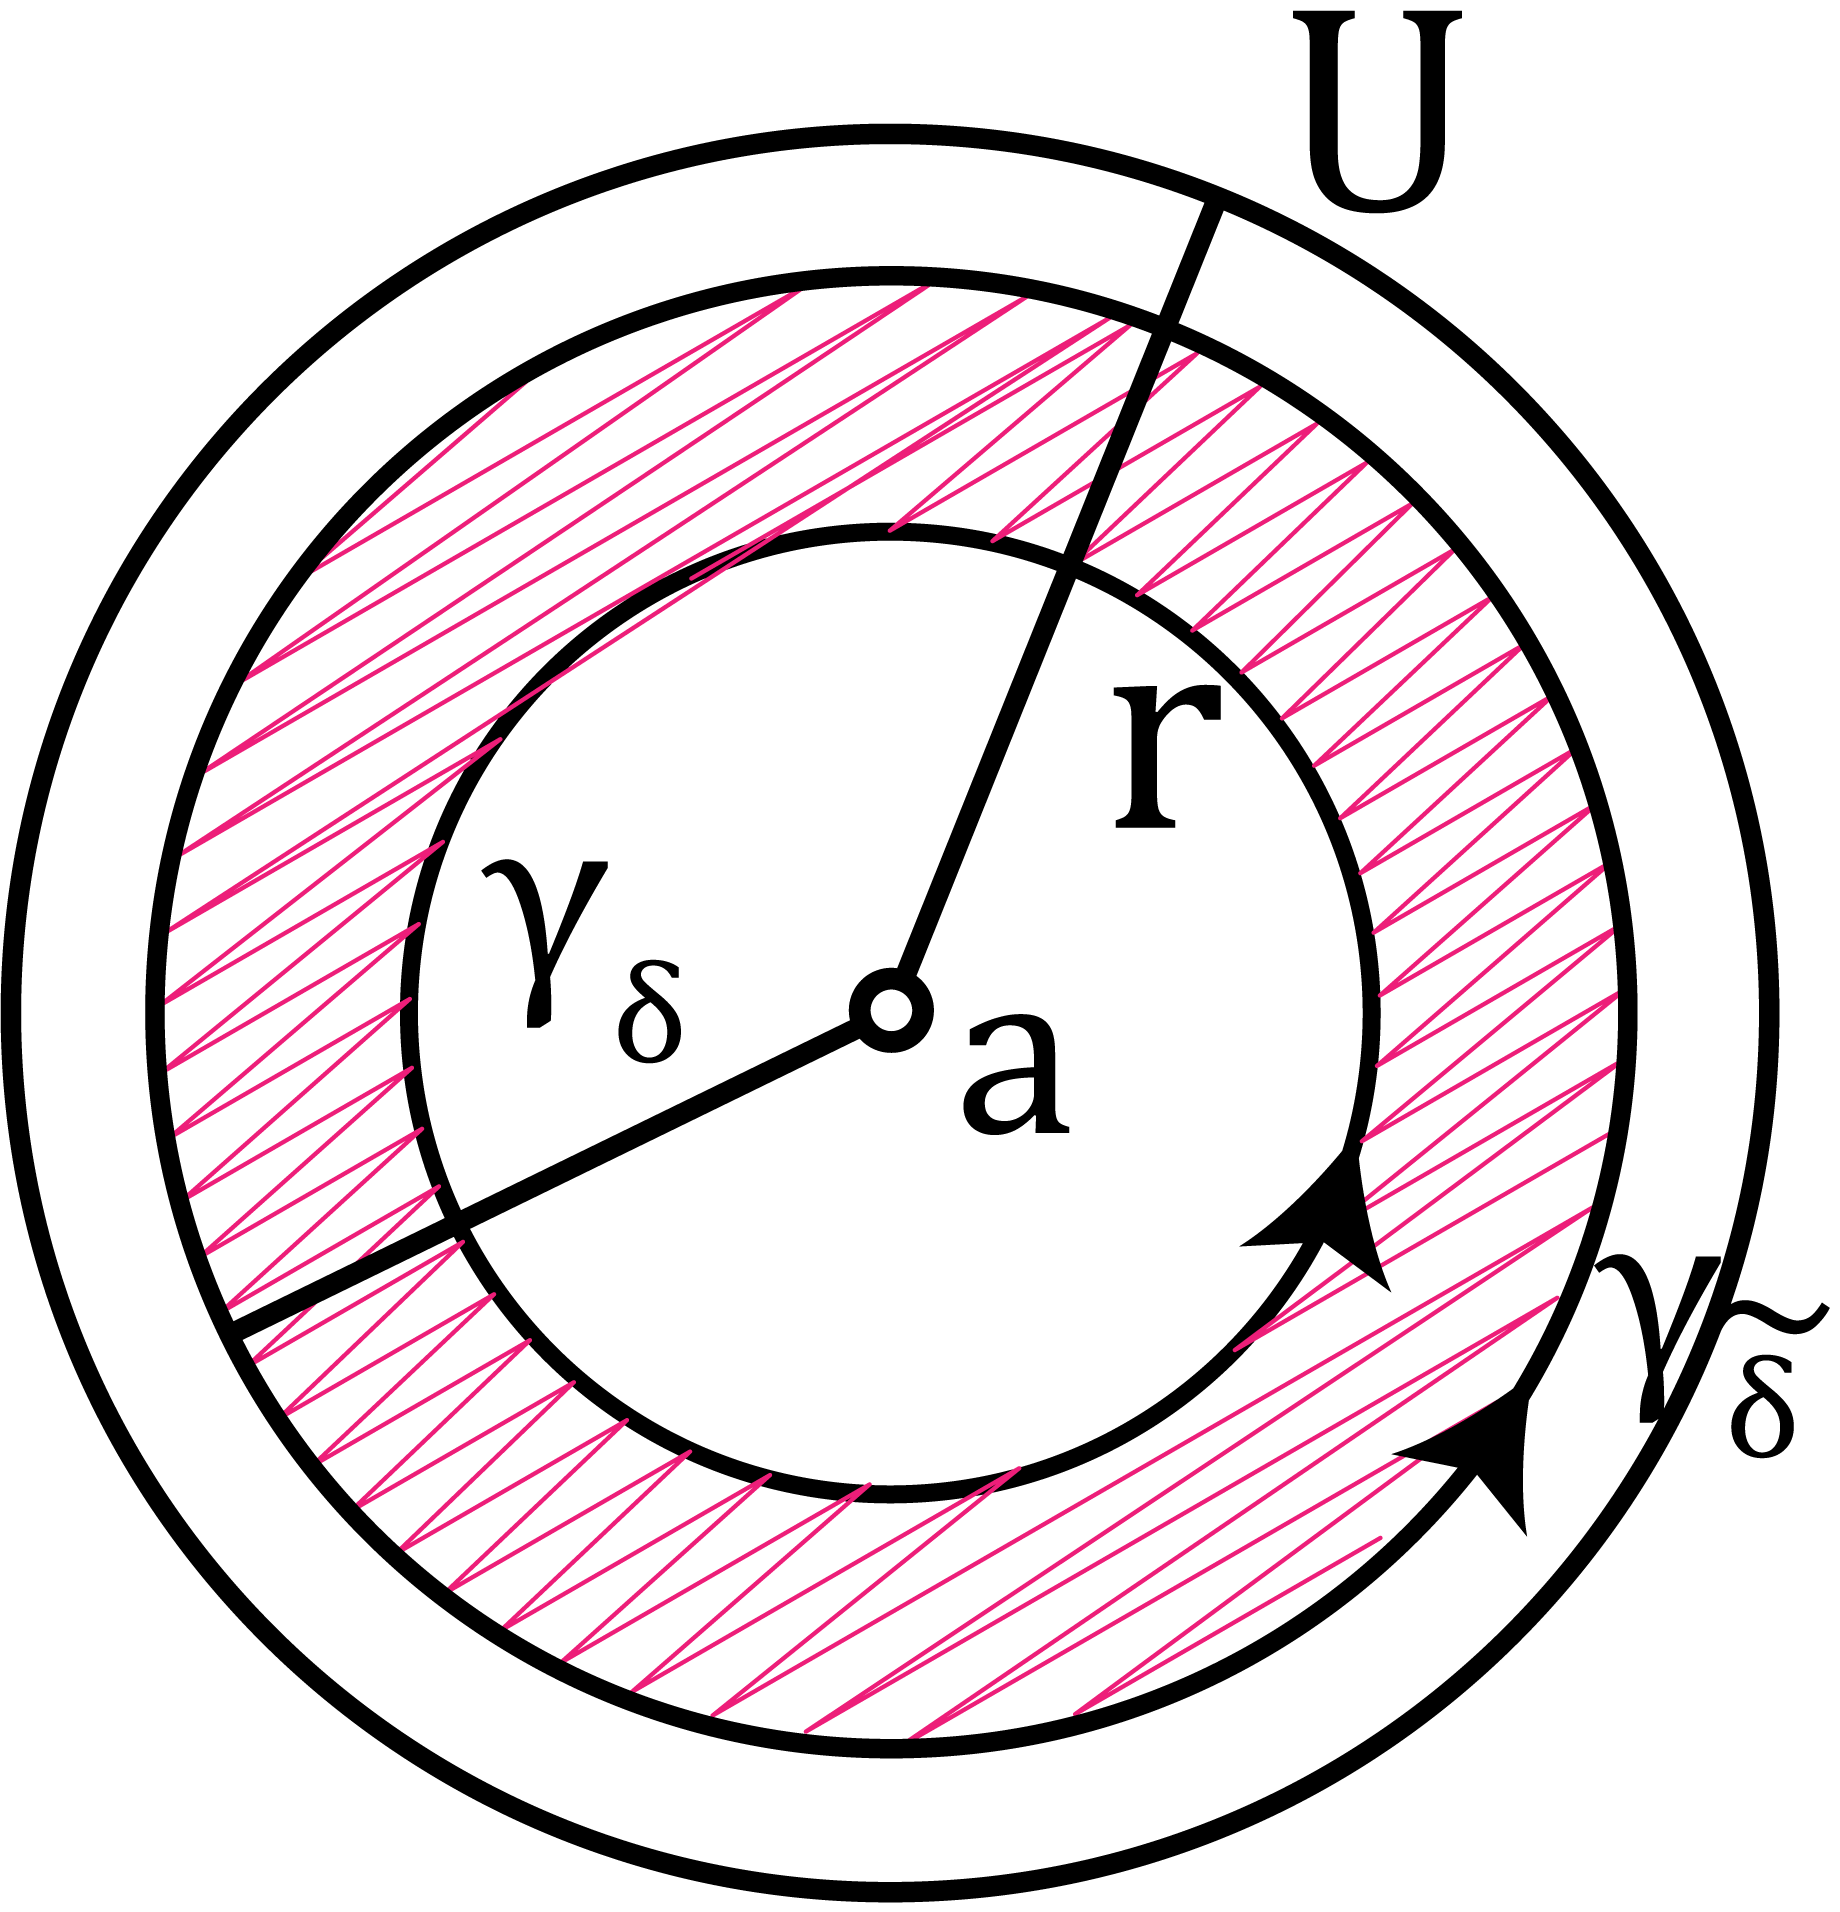
\includegraphics[width=4cm]{pics/13_3}
            \centering
        \end{figure}
    \end{Definition}

    \begin{remark}
        От $\delta$ опр. не зависит по т. Коши
        \[D = \{\delta \leq \abs{z - a} \leq \widetilde{\delta}\}\]
        \[\int_{\d D} f(\xi)d\xi = 0 = \int_{\gamma \widetilde{\delta}} - \int_{\gamma \delta}   \]
    \end{remark}

    \hline
    \[f(z) = \sum_{n = -\infty}^{+ \infty} c_n(z - a)^n   \q\text{ разл. в р.Л в окр т. } a \]
    \[res_af = \frac{1}{2\pi i} \int_{\gamma_\delta} \sum_{n = -\infty}^{+\infty} c_n(\xi - a)^n d\xi   \]
    На окр-ти $\gamma_\delta$ р.Л. сх. равномерно
    \[\Ra \text{ почл. проинт.}\]
    \[\gamma_\delta : \q \abs{\xi - a} = \delta\]
    \[\xi - a = \delta e^{it}, \q - \pi \leq t \leq \pi \]
    \[\int_{\gamma_\delta} (\xi - a)^n d\xi = i\int_{-\pi}^\pi \delta^n e^{int}\delta  e^{it}dt    \]
    \[= \begin{cases}
        0, & n \neq -1\\
        2\pi i   & n = -1
    \end{cases}\]
    \[res_af = c_{-1} \]

    \begin{Definition}
        \[res_af = c_{-1}, \text{ где  }c_{-1} \text{ - коэф. при } z^{-1} \text{ в разл. в р.Л. } f(z)   \]
        в прок. окр. т. $a$
    \end{Definition}

    \subsubsection{Вычисление вычетов}

    \begin{definition}
        \begin{enumerate}
            \item если $a$ - устр. ос. т. \q $a \in \CC \q (a \neq \infty)$
                \[c_{-1} = 0 = res_a f \]
            \item $a$ - полюс порядка 1 (простой полюс)
                \[f(z) = \frac{c_{-1} }{z - a} + c_0 + \text{ пр. часть р.Л.}\]
                \[res_a f = \lim_{z \to a} (z - a) \cdot f(z) \]
        \end{enumerate}
    \end{definition}

    \begin{definition}
        Если $a$ - полюс 1 порядка, причем
        \[f(z) = \frac{\varphi(z)}{\psi(z)}, \text{ где } \psi(a) = 0, \q \varphi(a) \neq 0\]
        \[(\text{т.о } a \text{ - ноль кр. 1 } \psi(z))\]
        \[\varphi \text{ - непр} \qq \psi \text{ - дифф.}\]
        \[res_a f = \lim_{z \to a} \frac{(z - a)\varphi(z)}{\psi(z)} = \lim_{z \to a}
        \frac{\varphi(z)}{\frac{\psi(z)}{(z - a)}}\]
        \[\lim_{z \to a} \frac{\psi(z) - \psi(a)}{z - a} = \psi'(a) \]
        \[res_a f = \frac{\varphi(a)}{\psi'(a)}\]
    \end{definition}

    \begin{Definition}
        \[a \text{ - полюс порядка }N\]
        \[f(z) = \frac{c_{-N} }{(z - a)^N} + ... + \frac{c_{-1} }{z - a} + c_0 + c_1(z - a) + ...\]
        \[g(z) = c_{-N} + c_{-N + 1}(z - a) + ... + c_0 (z - a)^N + ...  \]
        \[g \in H(\doted{U}_r(a)), \qq f(z) = \frac{g(z)}{(z - a)^N}\]
        \[g(z) = \sum_{k = 0}^\infty a_k (z - a)^k \qq c_{-1} = a_{N - 1} =
        \frac{g^{(N - 1)}(a) }{(N - 1)!}\]
        \[c_j = a_{j + N} \]
        \[res_a f = \lim_{z \to a} \frac{d^{N - 1}( (z - a)^N f(z))}{(N - 1)!dz} \]
    \end{Definition}

    \newpage
    \subsection{Теорема Коши о вычетах. Вычет в бесконечно удаленной точке}

    \begin{Theorem}[Коши о вычетах]
        \[\text{Пусть } f \in H(D\setminus \{z_1, z_2, ..., z_N\})\]
        и $f $ аналит на $\Gamma = \d D$
        %рисунок4
        \begin{figure}[H]
            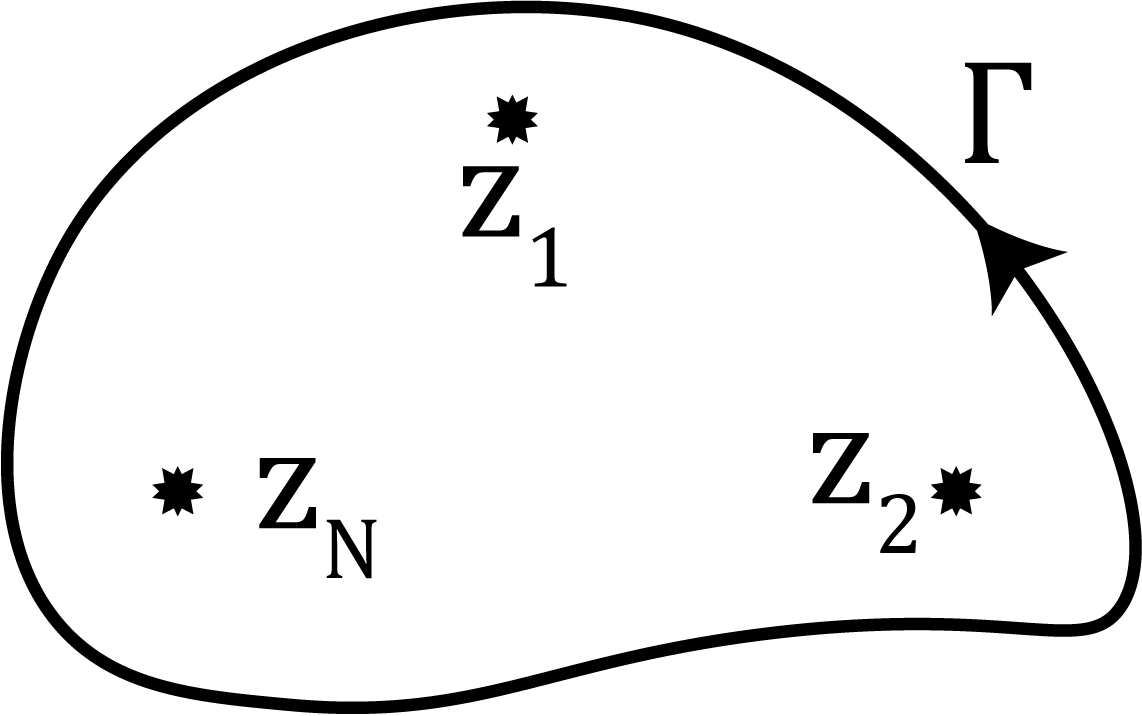
\includegraphics[width=4.5cm]{pics/13_4}
            \centering
        \end{figure}
        \[\text{Тогда } \int_{\Gamma} f(\xi)d\xi = 2\pi i \cdot \sum_{k = 1}^N  res_{z_k} f  \]
    \end{Theorem}

    \begin{Example}
        \[\int_{\abs{z} < 10}  e^{\frac{1}{z}}dz = 2\pi i\]
        \[e^{\frac{1}{z}}  = 1 + \frac{1}{z}  + \frac{1}{2z^2} + \frac{1}{3!z^3} + ...\]
        \[c_{-1} = res_0e^{\frac{1}{z}}  = 1 \]
    \end{Example}

    \begin{Proof}\
        %рисунок5
        \begin{figure}[H]
            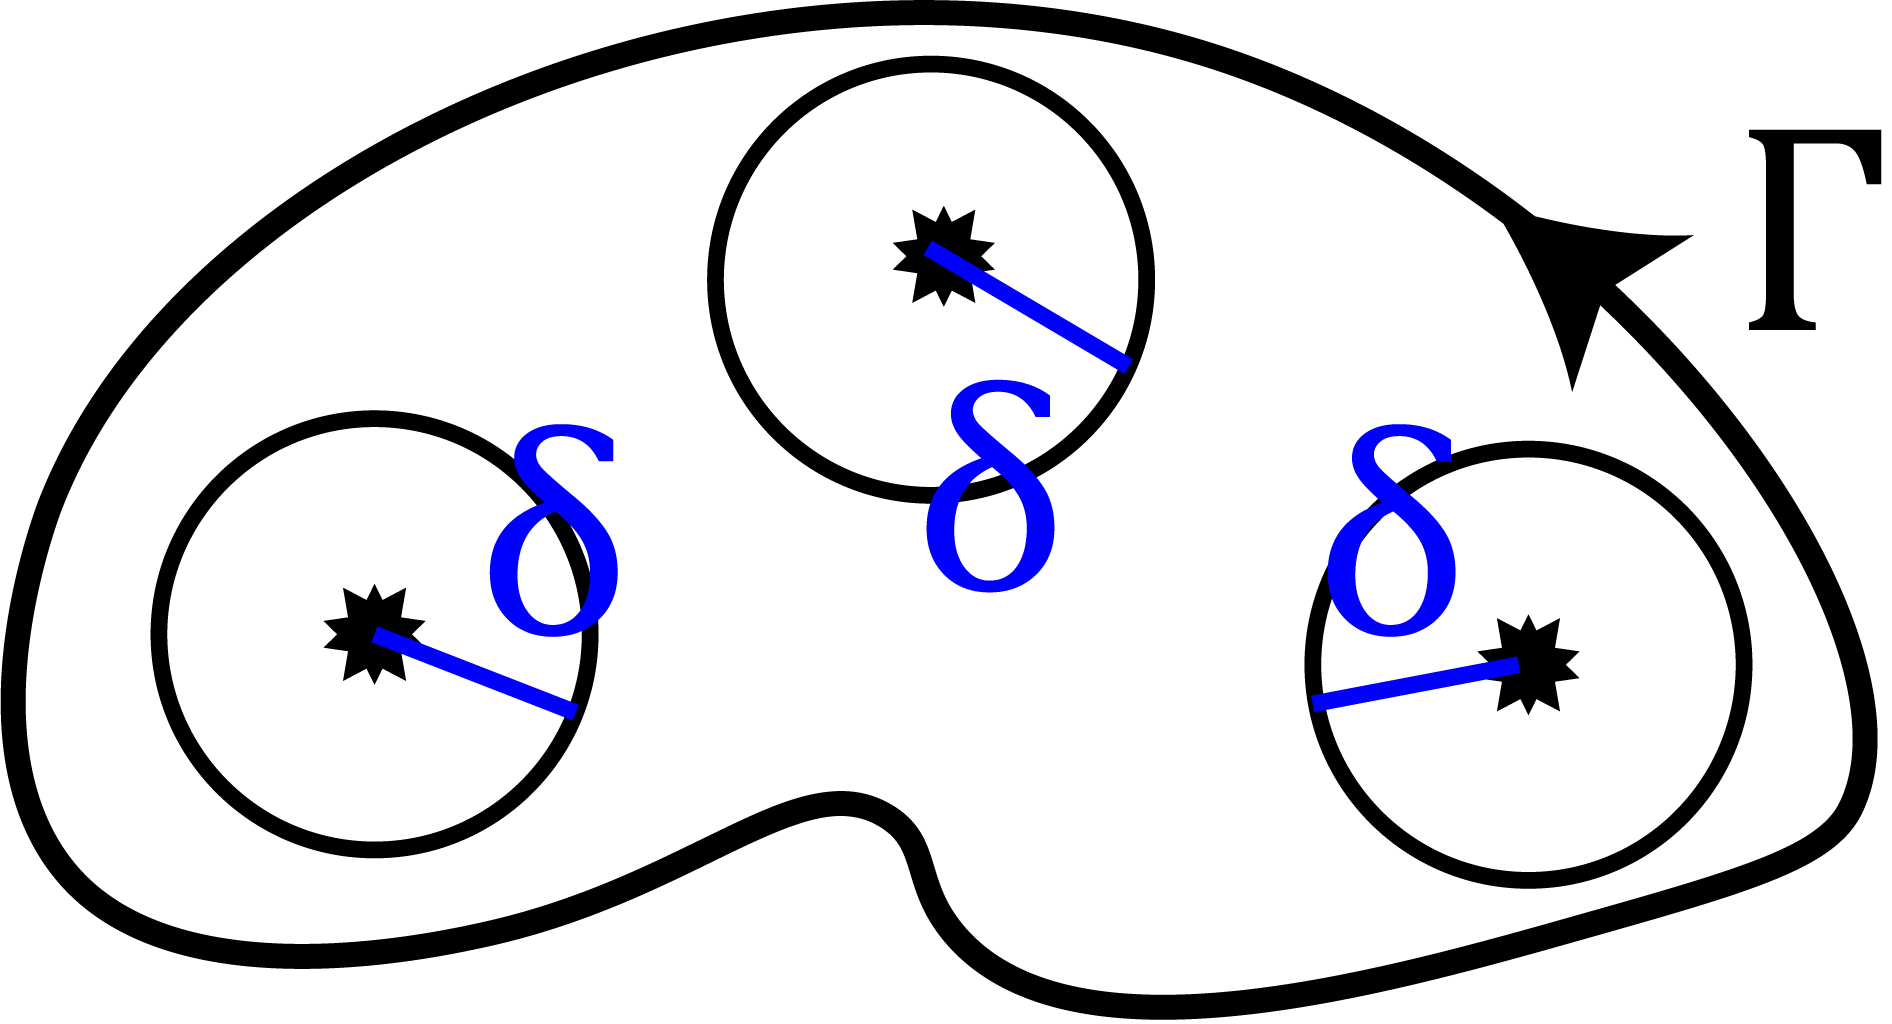
\includegraphics[width=4cm]{pics/13_5}
            \centering
        \end{figure}
        \[\widetilde{D} = D \setminus \bigcup_{k = 1}^N  \{z : \abs{z - z_k} \leq \delta\}\]
        \[\d \widetilde{D} = \Gamma \cup \bigcup_{k = 1}^N \gamma_\delta^k \qq
        \gamma_\delta^k = \{\abs{z - z_k} = \delta\}\]
        \[f \in H(\widetilde{D}) \Ra \int_{\d \widetilde{D}} f(\xi)d\xi = 0 \]
        \[\int_{\d \widetilde{D}} f(\xi)d\xi = \int_{\Gamma} f(\xi)d\xi -
        \sum_{k = 1}^N \int_{\gamma_\delta^k} f(\xi)d\xi = 0  \]
        По опр. $res_{z_k} f = \frac{1}{2\pi i} \int_{\gamma_\delta^k} f(\xi)d\xi  $
        \[\int_\Gamma f(\xi) d\xi = 2\pi i \sum_{k = 1}^N res_{z_k} f\]
        %рисунок6
        \begin{figure}[H]
            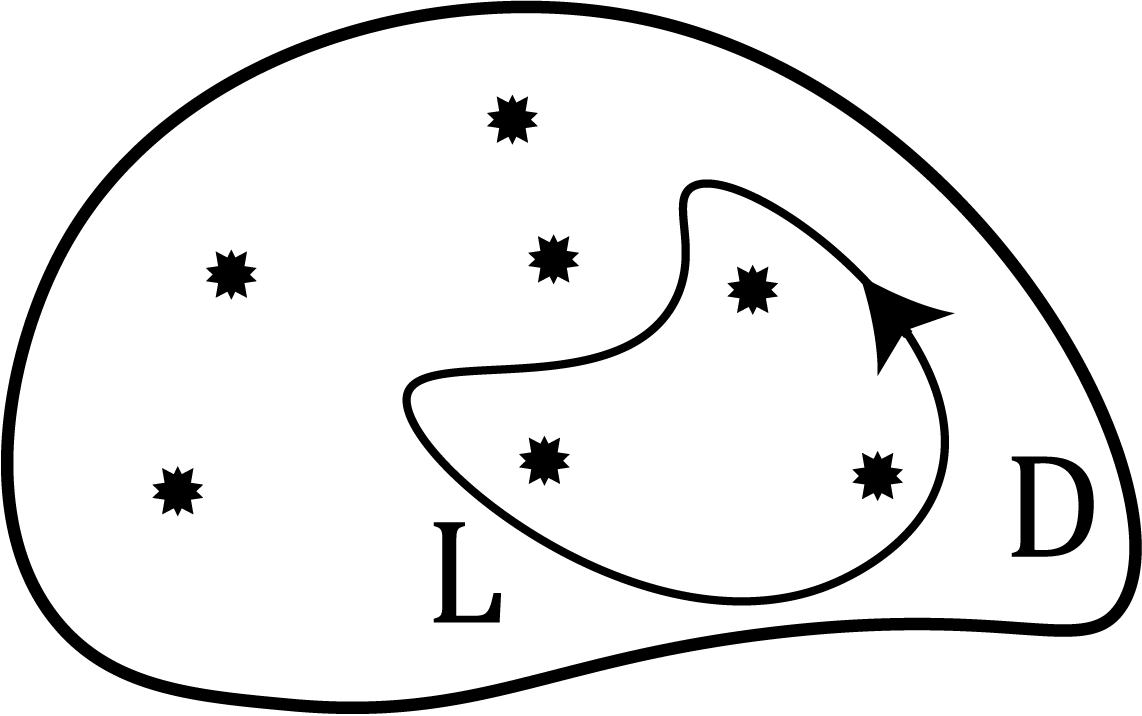
\includegraphics[width=4.5cm]{pics/13_6}
            \centering
        \end{figure}
        \[\int_{L} f(\xi)d\xi = 2\pi i \sum_{z_k \text{ внутри } L}  res_{z_k} f  \]
    \end{Proof}

    \newpage
    \subsubsection{Применение для вычисления нек. опр. инт-лов}

    \begin{Definition}
        \[\us{\text{рац. дробь (тригонометр.)}}{R(\cos t, \sin t)}\]
        \[\int_{-\pi}^\pi R(\cos t, \sin t)dt = \int_{\abs{z} = 1} R \left(\frac{z + z^{-1} }{2}, \
        \frac{z - z^{-1} }{2i}\right) \frac{dz}{iz} \]
        \[\cos t = \frac{e^{it} = e^{-it}  }{2}, \q \sin t = \frac{e^{it} - e^{-it}  }{2i} \q z = e^{it} \]
        \[dz = z \cdot i \cdot dt\]
    \end{Definition}

    \begin{Example}
        \[\int_0^\pi \frac{dt}{2 + \cos t} = \frac{1}{2} \int_{-\pi}^\pi \frac{dt}{2 + \cos t} =
        \frac{\pi}{\sqrt{3}}\]
        \[\int_{-\pi}^{\pi} \frac{dt}{2 + \cos t} = \int_{\abs{z} = 1} \frac{dz}{
        iz(2 + \frac{z + z^{-1} }{2})}   =  \frac{1}{i} \int_{\abs{z} = 1} \frac{2dz}{z^2 + 4z + 1} =   \]
        \[\frac{1}{i}\int_{\abs{z} = 1} \frac{2dz}{(z + 2 + \sqrt{3})(z + 2 - \sqrt{3})} =  \]
        %рисунок7
        \[= \frac{1}{i} 2\pi i \cdot res_{-2 + \sqrt{3}} \frac{2}{(z + 2 + \sqrt{3})(z + 2  -\sqrt{3})} =  \]
        \[ = 2\pi \lim_{z \to -2 + \sqrt{3}} \frac{2(z + 2 - \sqrt{3})}{(z + 2 + \sqrt{3})(z + 2 - \sqrt{3})} =
        \frac{4\pi}{2\sqrt{3}} = \frac{2\pi}{\sqrt{3}}\]
    \end{Example}

    \newpage
    \subsubsection{Преобразование Фурье рац. функции}

    \begin{Definition}
        \[ R(z) = \frac{P(z)}{Q(z)} \qq \text{ Пусть } Q(x) \neq 0 \q \forall x \in \R\]
        %рисунок8
        \[\text{ И }\abs{R(z)} \leq \frac{const}{\abs{z}^2} \qq \forall z : \abs{z} > R \qq R > 0\]
        \[(\deg Q - \deg P \geq 2)\]
        \[\hat{f}(\lambda) = \int_{-\infty}^{+\infty} f(x)e^{-i\lambda x}dx \text{ преобразование Фурье}   \]
        \[(V.P.) \q \int_{-\infty}^{+\infty} R(x) e^{i\lambda x} dx = \begin{cases}
            2\pi i \displaystyle \sum_{\Im z_k > 0}  res_{z_k}  (R(z)e^{i\lambda z}), & \text{ если } \lambda
            \geq 0\\
            -2\pi i \displaystyle \sum_{\Im z_k < 0} res_{z_k} (R(z)  e^{i\lambda z} ), & \lambda \leq 0
        \end{cases}   \]
        \[z_k \text{ - Нули } Q(z)\]
    \end{Definition}

    \begin{Example}
        \[\int_{-\infty}^{+ \infty} \frac{1}{(x^2 + 1)^2} \cos 3x dx =
        \real \int_{-\infty}^{+\infty} \frac{e^{i3x} }{(x^2 + 1)^2} dx =  \]
        \[= \real (2\pi i \cdot res_i \frac{e^{i3z} }{(z^2 + 1)^2})\]
        %рисунок9
        \[f(z) = \frac{e^{i3z} }{(z^2 + 1)^2} \q z_1 = i \text{ --- полюс порядка 2}\]
        \[\frac{1}{f(z)} = \frac{(z + i)^2(z - i)^2}{e^{i3z} }\]
        \[h(z) = \frac{(z + i)^2}{e^{i3z} }\]
        \[res_i f = \lim_{z \to i} \frac{d ((z - i)^2 f(z))}{1! dz} =
        \left(\frac{e^{i3z} }{(z + i)^2}\right)'\bigg|_{z = i} =  \]
        \[= \frac{3i e^{3iz}(z + i)^2 - 2(z + i)e^{3iz}  }{(z + i)^4} \bigg|_i =
        \frac{-3ie^{-3}4 - 4ie^{-3}  }{16} = -ie^{-3} \]
        \[\int_{-\infty}^{+\infty} \frac{\cos 3x}{(x^2 + 1)^2}dx =
        \real (2\pi i (-ie^{-3} )) = 2\pi e^{-3} \]
    \end{Example}

    \begin{Proof}
        %рисунок10(он 7)
        \begin{figure}[H]
            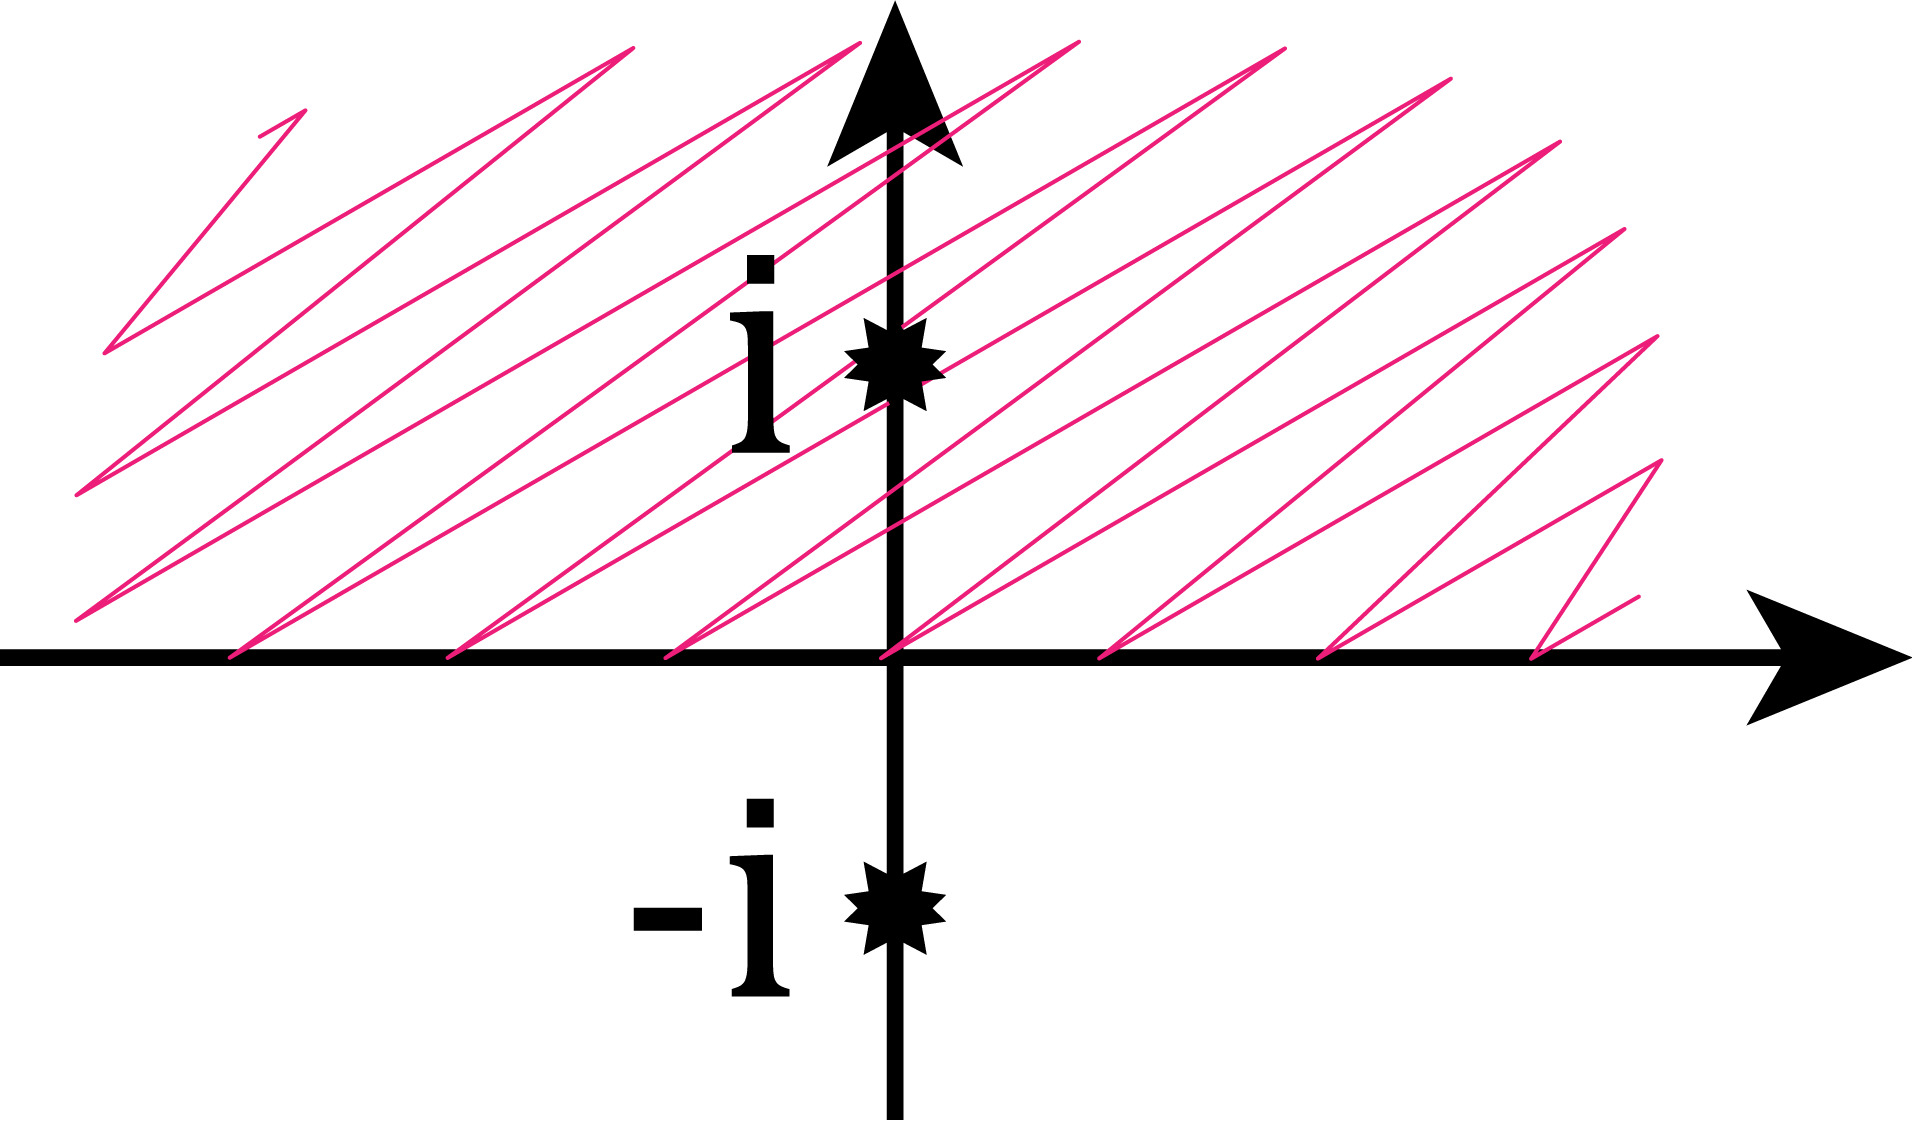
\includegraphics[width=3.5cm]{pics/13_7}
            \centering
        \end{figure}
        \[V.P. \q \int_{-\infty}^{+\infty} = \lim_{A \to +\infty}  \int_{-A}^{A}    \]
        \[C_A : \xi = A e^{it}, \q 0 \leq t \leq \pi \]
        \[\Gamma_A \text{ --- контур, сост из отр. } [-A, A] \q \text{ и полуокр } C_A\]
        \[\text{Пусть } A > R \text{ и такое, что все нули } Q \q z_k : \abs{z_k } < A\]
        %рисунок11(наверное, теперь все точки внутри)
        \begin{figure}[H]
            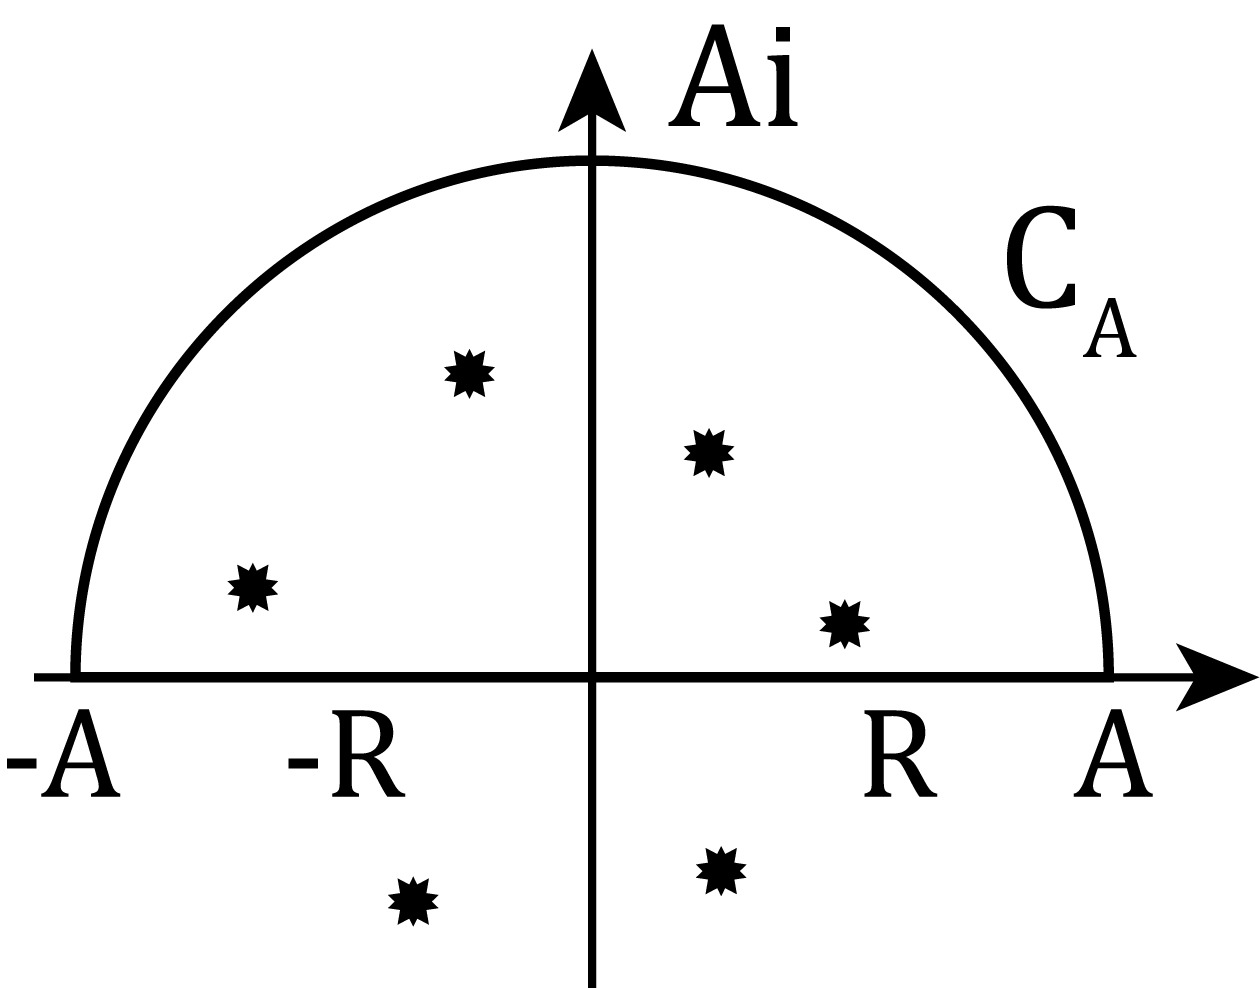
\includegraphics[width=4cm]{pics/13_8}
            \centering
        \end{figure}
        \[\int_{\Gamma_A} R(\xi)e^{i\lambda \xi} d\xi = 2\pi i \sum_{\Im z_k > 0} res_{z_k}
        (R(z)e^{i\lambda z} )\]
        \[= \int_{C_A} + \int_{-A}^A  \]
        \[\abs{\int_{C_A} R(\xi)e^{i\lambda \xi}d\xi  } = \abs{\int_0^{\pi} R(A e^{it} )e^{i\lambda A e^{it} }
        A e^{it} i dt } \leq  \]
        \[\leq \int_0^\pi \abs{R(Ae^{it} )}\abs{e^{i\lambda A\cos t - \lambda A \sin t} }A dt \leq
        \int_0^\pi \frac{const}{A^2}e^{-\lambda A \sin t} A dt = \]
        \[= \frac{1}{A} \int_0^\pi const \cdot e^{-\lambda A \sin t}dt \us{A \to \infty}{\to } 0 \]
        \[\int_{-A}^A R(\xi)e^{i\lambda \xi} d\xi = 2\pi i \sum_{\Im z_k > 0} (R(z)e^{i\lambda z} ) \text{
        не зависит от }  A\]
        \[\Ra \lim_{a \to \infty} \int_{-A}^A R(x)e^{i\lambda x} dx = (V.P.) \int_{-\infty}^{+ \infty}
        R(x)e^{i\lambda x}dx = 2\pi i \sum_{\Im z_k > 0} res_{z_k}   \]
    \end{Proof}

    \newpage
    \subsection{Лемма Жордана. Два следствия}

    \begin{Lemma}[Жордана]
        \[f \text{ - непр на } \{z : \Im z \geq 0; \q \abs{z} \geq R\}\]
        \[C_A : \q \xi = A e^{it} \qq 0 \leq t \leq \pi \]
        %рисунок12
        \begin{figure}[H]
            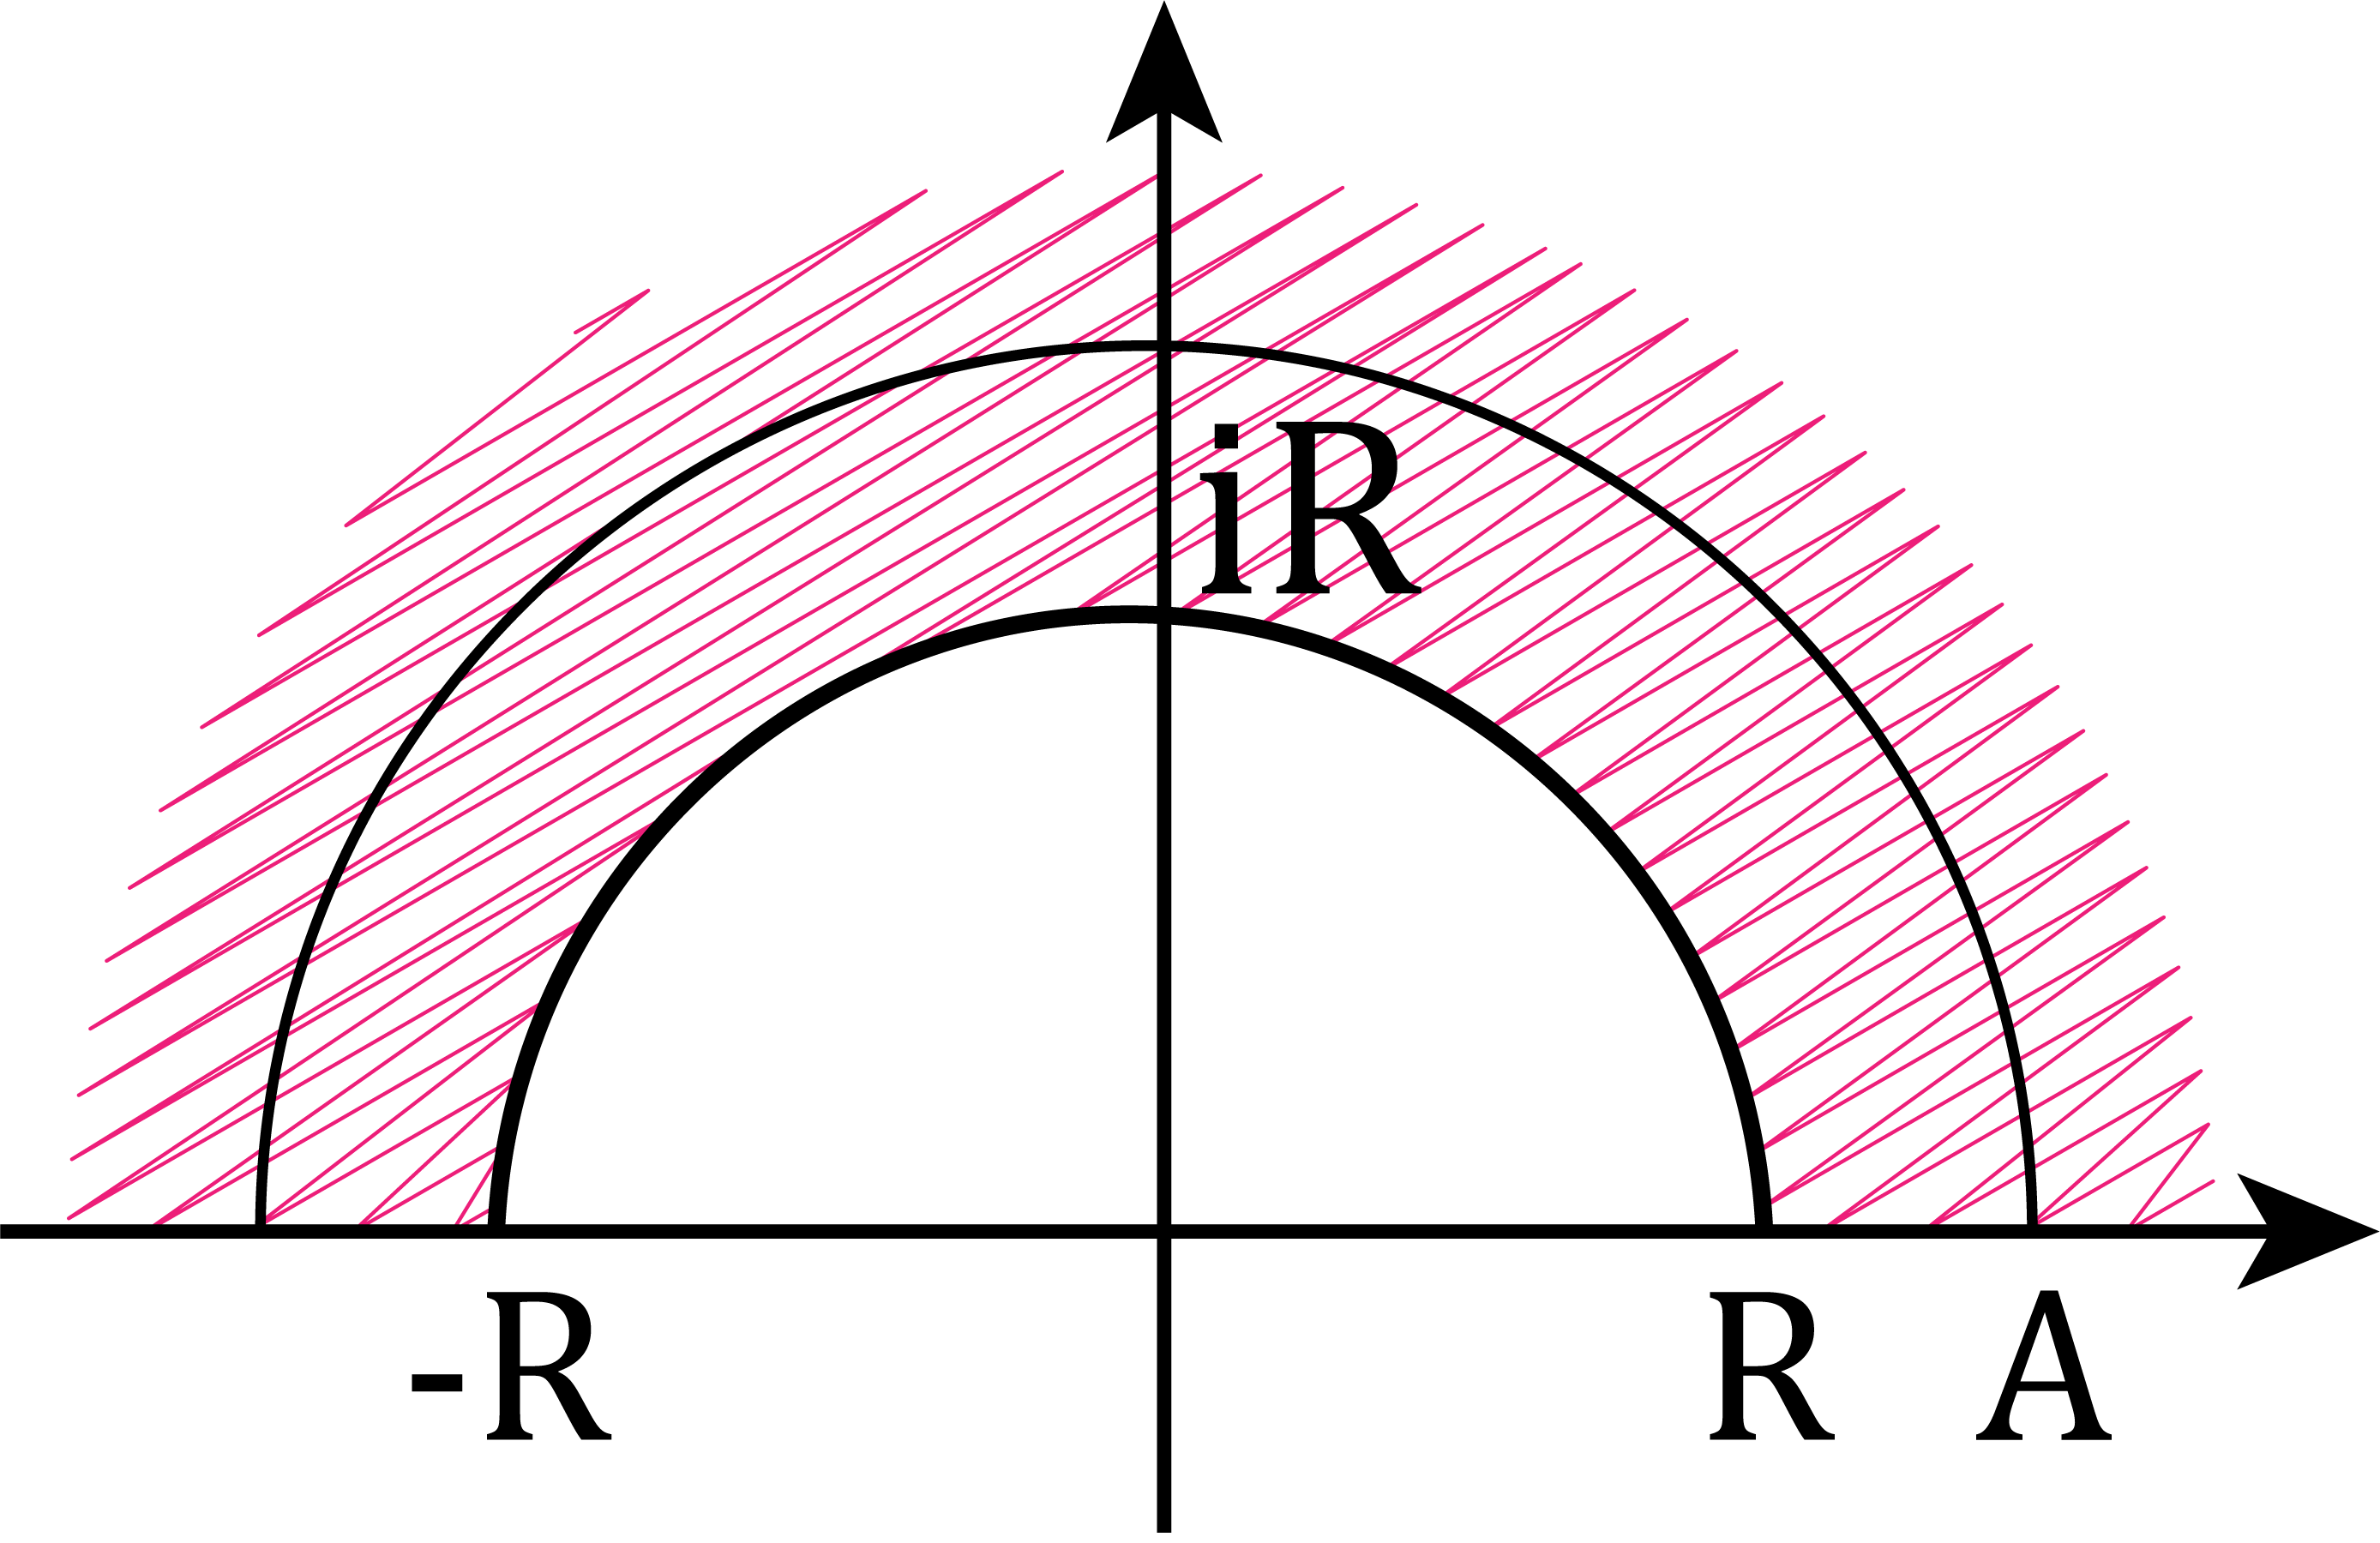
\includegraphics[width=5cm]{pics/13_9}
            \centering
        \end{figure}
        \[M_A = \max_{0 \leq t \leq \pi}  \abs{f(Ae^{it} )} \us{A \ra 0}{\to} 0\]
        \[\text{Тогда } \int_{C_A} f(\xi)e^{i\lambda \xi} d\xi \to  0 \qq \forall \lambda \geq 0  \]
    \end{Lemma}

    \begin{Proof}
        \[\abs{\int_{C_A} f(\xi)e^{i\lambda \xi} d\xi} = \abs{\int_{0}^\pi f(Ae^{it} )Ae^{i\lambda Ae^{it} }
        ie^{it}dt }  \leq  \int_0^\pi \abs{f(Ae^{it} )}e^{-A \lambda \sin t}Adt \leq  \]
        \[\leq M_A \cdot A\int_0^\pi e^{-A\lambda\sin t}dt \q (\star) \]
        %рисунок12
        \begin{figure}[H]
            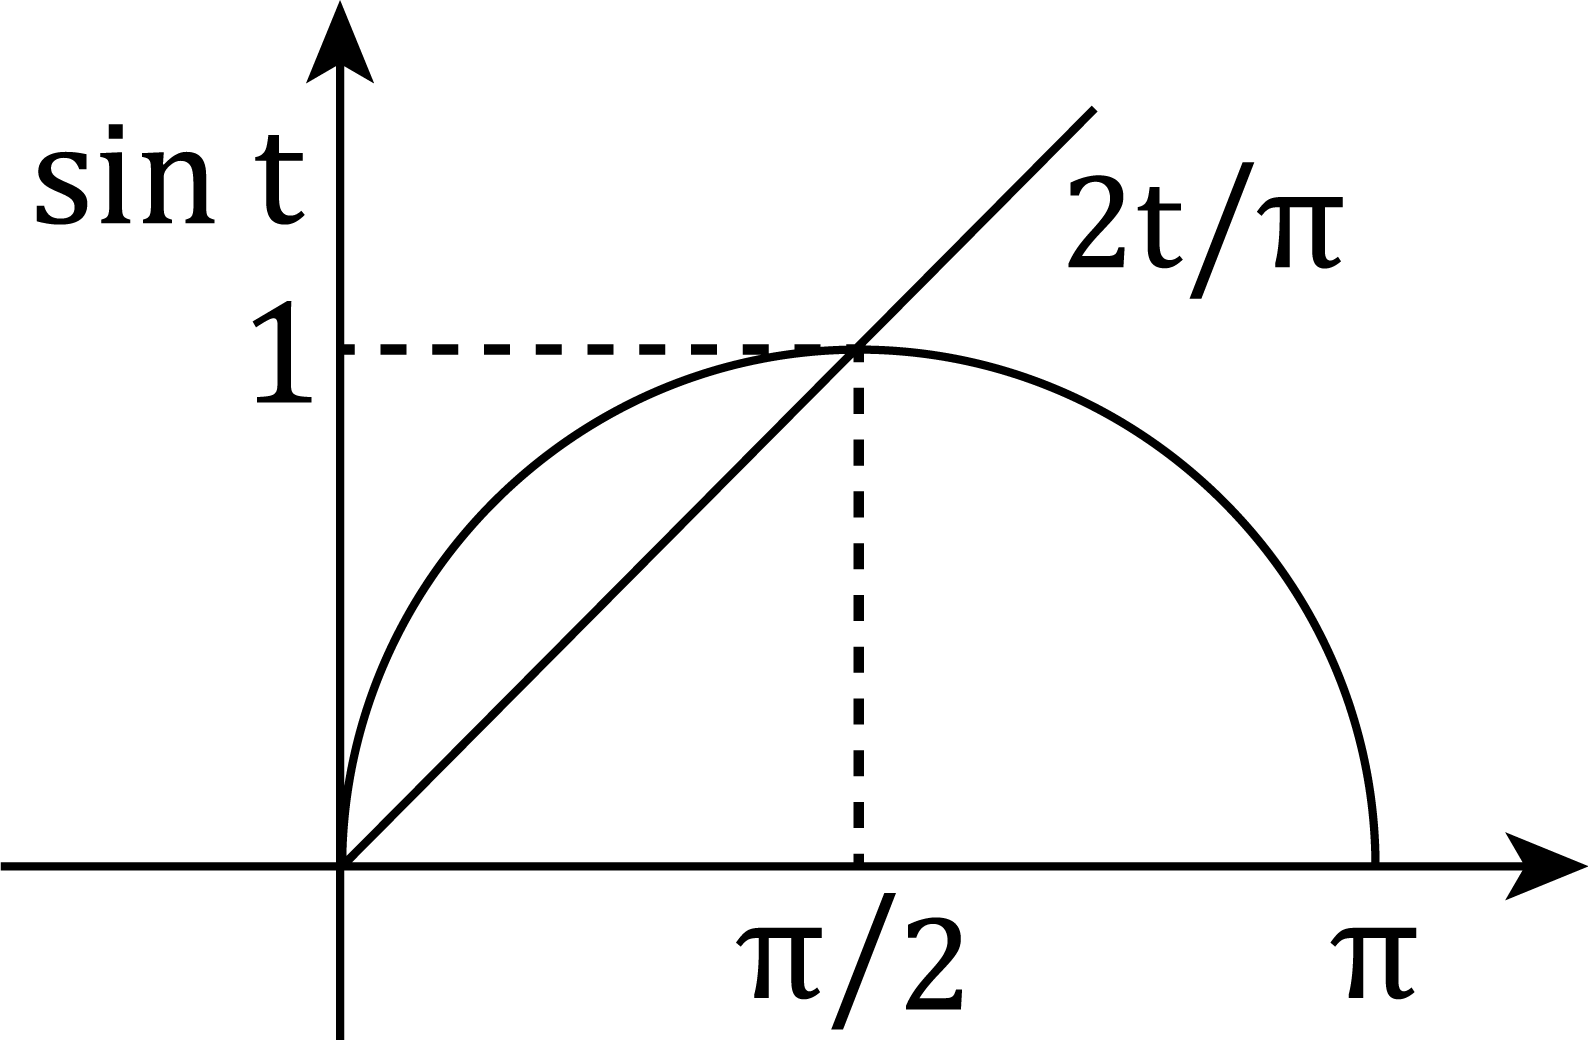
\includegraphics[width=5cm]{pics/13_10}
            \centering
            \caption{$\sin t \geq \frac{2t}{\pi}$}
        \end{figure}
        \[\int_0^\pi \us{\text{симм. отн. $t = \frac{\pi}{2}$}}{e^{-A \lambda \sin t}} dt =
        2 \int_{0}^{\frac{\pi}{2}} e^{-A \lambda \sin t} dt \leq  2 \int_0^{\frac{\pi}{2}}
        e^{-A \lambda \frac{2t}{\pi}}dt =     \]
        \[= -2 \frac{\pi}{2 \lambda A} (e^{-A\lambda} - 1) \leq \frac{\pi}{\lambda A} \]
        \[(\star) \q \abs{\int_{C_A} f(\xi)e^{i\lambda \xi} d\xi  } \leq
        M_A \cdot \const \us{ A \to  \infty}{\to } 0 \]
    \end{Proof}
\end{document}
